%%%%% Beginning of preamble %%%%%

\documentclass[12pt]{article}  %What kind of document (article) and what size}

\usepackage{amssymb, amsmath, amsthm}
\usepackage{bbm}
\usepackage{graphicx}
\usepackage{biblatex}
\addbibresource{references.bib}
\usepackage[margin=1in]{geometry}
\graphicspath{ {report-figures/} }
\usepackage{subcaption}
\parskip = 0.1in
\title{MA 750 - Final Project}
\author{
  Nate Josephs\\
  \and
  Matthew Wiens 
  \and 
  Ben Draves
}
\begin{document}

\maketitle 
\begin{abstract} One of the most fundamental tasks in Statistics is to understand the relationship between two random variables, $X,Y$, via an unspecified function $Y = f(X)$. Typically, $f(\cdot)$ is unknown and must be estimated from data relating $X$ and $Y$. Estimating $f(\cdot)$ using maximum likelihood yields no meaningful solution when we consider \textit{all} functions. Hence statisticians turn to estimating $f\in\mathcal{F}$ where $\mathcal{F}$ is a function space with some structure that provides meaningful solutions to the problem at hand. In most cases however, these function spaces are fixed, with no regard to the sample from which we are trying to infer $f$. In order to utilize all information inherent in the data while still imposing structure on $\mathcal{F}$, \textit{Sieve Estimation} allows $\mathcal{F}$ to grow in complexity as $n$ increases. Heuristically, as $n$ increases, we attain a more robust understanding of $f$ and should allow our modeling procedure to consider more complex forms of $f$. Sieve achieves this by introducing more complex functions to $\mathcal{F}$ as $n$ increases. Here, we consider the function space $$\mathcal{F}_n = \Big\{g(x): g(x) = \sum_{d=0}^{D}\alpha_d\phi_d(x)\Big\}$$ for basis function $\phi_d$ and where $D\to\infty$ as $n\to\infty$. We focus our efforts on estimating $D$ as a function of the data. This report is organized as follows; in sections 1 and 2 we summarize some of the foundational results on Sieve estimation and introduce notation used throughout the report. In section 3 we introduce the theoretical optimal estimate of $D$ and a data dependent solution to this infeasible problem. In section 4 we provide a simulation experiment and apply this estimator in section 5 with a real data application. 
\end{abstract}

\section{Introduction}
\section{Development of Sieves Estimation}

\subsection{Series Estimators}
Sieve estimators are a general class of estimators that can applied to a number of nonparametric problems such as density estimation and regression. Within this framework, several models from the econometric literature have been developed, addressing tasks such as logistic regression, imputation techniques, and measurement error. While sieves is a general framework, we will focus on a sieve estimation for nonparametric regression. 

A sieve estimator for the unknown mean function $g(x)$ in a regression model is defined by a \textit{sequence} of functions approximating $g(x)$. With additional constraints such as the models should have finite dimension and the complexity (i.e. dimension) should increase as n increases, the most natural choice for the estimator is given by the \textit{series estimator} 
$$ \hat{g}(x) = \sum_{d=0}^{D} \alpha_{d} \phi_{d}(x)$$ 
This formulation leads to traditional problems in linear models, so given the dimension of the model and a choice of basis function, finding the coefficients $\alpha$ has well known solutions. The constraints in the formulation are light; namely the choice of basis function must approximate functions in $L^2$, among other typical constraints for the regression problem.  For completeness, examples of non linear sieves are Neural Networks, or penalized sieve estimators\cite{Chen}. 

Given the sieve estimator defined as a series, there are two choices to be made: the dimension of the model, and the choice of basis function.  $D$ must be data dependent to scale the complexity of the estimator with the data. Therefore, for now we will assume there is an algorithm to choose $D$ which produces a $D_{opt}$, for some sense of optimality. There are a number of choices for the basis functions, and we will highlight just a few possibilities here. We will discuss optimal choices of dimension in the following section. 

\subsection{Basis Functions}

One popular choice of functional estimator is given by the series estimator with polynomial basis functions. Within the polynomial class, choices of coefficients uniquely determine the exact form for the estimate. For example the coefficient vector $\textbf{c} = [0,0 \ldots, 1]$ would correspond to a basis of $\{x^{k}: k = 0,1,2,\ldots\}$. The Hermite Polynomials would correspond to another choice of $\textbf{c}$, which have desirable theoretical properties such as othronormality. While a powerful class of estimators, polynomial basis functions are not a natural choice when $g(x)$ goes to zero at $\pm \infty$. Using a Fourier Series resolves this issue, which again highlights the importance of an appropriate choice of basis function in function estimator. With several applications in signal processing, the Fourier basis is proven to be a natural choice to approximate periodic functions. Lastly the Gaussian basis set, given by $\{\varphi^{(d)}:d= 0,1,2,\dots\}$ where $\varphi^{(d)}$ is $dth$ derivative of the Normal density has several similar properties of the Fourier basis. Moreover, we see that these functions have a natural probabilistic interpretation (as do the Hermite Polynomials) which could be quite useful in inferential settings. The functional forms of these basis sets are given in the Table \ref{tab:basis}. 

\begin{table}[h]
\begin{center}
\begin{tabular}{|c|c|}
\hline
Basis Functions & Functional Form\\
\hline
Polynomaials & $\sum_{i=0}^{d} c_d x^d$\\
Fourier &$a~cos(\pi d x) + b~sin(\pi d x)$\\
Guassian &$\varphi^{(d)}(x)$\\
\hline
\end{tabular}
\caption {Proposed series estimators with basis function $\phi$ for $\hat{g}(x)$ }
\label{tab:basis}
\end{center}
\end{table}
Where $\phi^{(d)}(x)$ is the $dth$ derivative of the Normal density, which will be the Normal density with coefficients  of the $dth$ Hermite polynomial. Like the Fourier Series, the Gaussian series estimator has the nice property that it goes to zero at $\pm \infty$.

Other common choices for the basis function are Splines and Wavelets.  Different splines can be used as the sieve estimator, however the exact form and behavior depends on the choice of spline and the number of free parameters it has.  This result can be shown by considering a constrained optimization problem over the squares of the Dth derivatives of the class of potential sieve estimators. Also note that the choice of basis in the univariate case extends naturally to the multidimensional case, where the multivariate basis is constructed as a tensor produce of the univariate basis\cite{Chen}.

With the setup of a series estimator with a choice of dimension and basis function the sieve estimator has a number of similarities to the Kernel Density estimation problem.  In both cases there are two choices to be made, one parameter that controls the bias variance tradeoff, and a second parameter that is related to underlying beliefs about the model.  So the bandwidth in the Kernel estimation problem is analogous to the choice of dimension. Intuitively, as the dimension increases or the bandwidth decreases the estimator is more sensitive to local behavior and produces a rougher estimate. Similarly, the choice of the Kernel is analogous to the choice of basis function; the choice impacts the final model and exact statistical properties of the estimator, yet is less interesting because any reasonable choice of basis function or kernel function produces a similar estimate. 

\subsection{Analysis of Series Estimators}

To begin our formal analysis of the series estimator suppose we have some function $f(x)$ that can be well approximated by a series estimator. That is we can write $$y_i\equiv f(x_i) + e(x_i)= \sum_{d=0}^{\infty}\phi_{d}(x_i)\alpha_d + e(x_i)$$
where $\{\phi_d\}_{d=0}^{D}$ is a set of orthogonal basis functions and $\alpha_d$ are coefficients. Then the \textit{sieves} estimator for this function is given by $$\hat{f}(x_i) = \sum_{d=0}^{D}\phi(x_i)\alpha_{d} = \phi^{T}(x_i)\alpha$$where $\phi^{T}(x_i) = (\phi_{0}(x_i), \phi_{1}(x_i),\ldots, \phi_D(x))^{T}$ and $\alpha = (\alpha_0, \alpha_1, \ldots, \alpha_D)$. Now organizing our matrices as follows 

$$Y = \begin{bmatrix}Y_1\\ Y_2\\\vdots\\Y_n\end{bmatrix}, P_D = \begin{bmatrix}\phi_0(x_1) & \phi_1(x_1) & \ldots & \phi_{D}(x_1)\\\phi_0(x_2) & \phi_1(x_2) & \ldots & \phi_{D}(x_2)\\\vdots & \vdots & \ddots & \vdots \\\phi_0(x_n) & \phi_1(x_n) & \ldots & \phi_{D}(x_n)\\\end{bmatrix}, \alpha = \begin{bmatrix}\alpha_0\\\alpha_1 \\\vdots\\\alpha_D\end{bmatrix}, e =\begin{bmatrix}e(x_1)\\e(x_2)\\\vdots\\e(x_n)\end{bmatrix}$$ we can write our model as $$Y = P_D\alpha + e$$
Seeing this a linear function in $P_D$ gives rise to our OLS estimator of $\alpha$ $$\hat{\alpha} = (P_D^{T}P_D)^{-1}P_D^{T}Y$$ From here we see that our estimates are given by $$\hat{f}(x_i) = \phi^{T}(x_i)\hat{\alpha}$$
Due to the arsenal of statistical techniques for the linear regression model, we can extend this estimation procedure to account for correlated errors, weighted error structure, or even random effects. Now notice, that in the linear model framework these estimates would result in unbiased best estimates of the coefficients $\alpha$, \textit{given that we specify $D$ correctly}. In the case were we do not specify the mean function correctly (i.e. misspecifcy $D$), our estimate become unbiased and the variance also increases. This again highlights in the importance of correct estimation of the dimension of the series estimator which we discuss in the proceeding section. 
\section{Estimating the Dimension $D$}

\subsection{Mean Integrated Squared Error}
In this framework, we introduce two types of error. The first is given by the error of the approximation. This is, how well the series estimator matches the true underlying function. We will define this error by $$r(x) = \phi^{T}(x)\alpha - f(x)$$
(\textit{Notice that these are the true coefficient values}). The other source or error is of course the random variation around the true regression function. We will call this the residual error, $\epsilon(x_i)$. Then we see that from the original model $y_i = f(x_i) + e_i(x_i)$ that we can decompose the error as 
$$e_i(x_i) = \epsilon(x_i) + r(x_i)$$
As we vary $D$ we greatly reduce the variance in $r(x_i)$ as the more complex model will always account for more variance. But we need to be careful to ensure that the model is only reducing $r(x_i)$ not $\epsilon(x_i)$. To try and find an analytical choice of $D$, we will find the Mean Integrated Squared Error (MISE). First consider the following expansion. 
\begin{align*}
\hat{f}(x) - f(x) &=  \phi^{T}(x)\hat{\alpha} - f(x)\\
&= \phi^{T}(x)\hat{\alpha} - \phi^{T}(x)\alpha + \phi^{T}(x)\alpha- f(x)\\
&= \phi^{T}(x)\hat{\alpha} - \phi^{T}(x)\alpha + r(x)\\
&= \phi(x)\phi^{T}(x)\left(\hat{\alpha} - \alpha\right) + r(x)\\
&
\end{align*}{}
Assume that the underlying $X$ distribution is $g$. Then 
\begin{align*}
MISE(D) &=\int (\hat{f}(x) - f(x))^2 g(x)dx\\
&= \int \left(\phi^{T}(x)\left(\hat{\alpha} - \alpha\right) + r(x)\right)^2g(x)dx\\
&= \int r(x)^2g(x)dx + 2(\hat{\alpha} - \alpha)\int \phi^{T}(x)r(x)g(x)dx + (\hat{\alpha} - \alpha)^{T}\int \phi(x)\phi^{T}(x)g(x)dx (\hat{\alpha} - \alpha)\\
&= E(r^2(x)) + 2(\hat{\alpha} - \alpha)E(\phi^{T}(x)r(x)) + (\hat{\alpha} - \alpha)^{T}E(\phi(x)\phi^{T}(x))(\hat{\alpha} - \alpha)
\end{align*}
Now recall that the $r(x)$ was a projection error during our OLS estimate of $\alpha$. Therefore, $r(x)$ and $\phi^{T}(x_i)$ exists in orthogonal spaces. Hence $E(\phi^{T}(x)r(x)) = 0$. Moreover, since $\phi$ is a collection of orthogonal functions the off diagonal elements of $E(\phi(x)\phi(x)^T)$ are all zero. This gives 
\begin{align*}
MISE(D) &= E(r^{2}(x)) + \text{tr}\Big[(\hat{\alpha} - \alpha)^TE(\phi(x)\phi(x)^T)(\hat{\alpha} - \alpha)\Big]\\
&= E(r^{2}(x)) + tr\Big[E(\phi(x)\phi(x)^{T})E\left((\hat{\alpha} - \alpha)(\hat{\alpha} - \alpha)^{T}\right)\Big]
\end{align*}
Now according to Hansen 2012 with $E(e(x)^2|x) = \sigma_x^2$, $\mathcal{Q} = E(\phi(x)\phi^T(x))$ and $\Omega = E(\phi(x)\phi^T(x)\sigma_x^2)$ due to the asymptotic behavior of this quantity we have 
$$MISE(D)\simeq E(r^2(x)) + \frac{1}{n}tr\left(\mathcal{Q}^{-1}\Omega\right)$$
Now, if we assume homoscedasticity, we see that $\Omega = \sigma^2\mathcal{Q}$. So plugging into the equation above we see that 
$$MISE*(D)\simeq E(r^2(x)) + \frac{1}{n}tr\left(\sigma^2\mathcal{Q}^{-1}\mathcal{Q}\right) = E(r^2) + \frac{\sigma^2}{n}\dim(\mathcal{Q}) = E(r^2(x)) + \frac{\sigma^2 D}{n}$$
Hansen 2012 then show that $$MISE*(D) = MISE(D)(1 + o(1))$$ so $MISE*$ is close to $MISE$. But notice, even in this simple case we still require estimation of $r(x)$, which is directly related to the estimation of the true regression mean function $f(x)$ which is what we started to estimate in the first place. Therefore, while an excellent theoretical tool, using $MISE*$ in practice is infeasible. We will, however, use this theoretical exercise to inform our data dependent choices of $D$ which we give in the following sections.

\subsection{Prediction Squared Error}

As we have seen, MISE does not offer a feasible solution for selection $D$. Instead of MISE, one may be interested in calculating the Predicted Square Error (PSE) in order to find the optimal dimension with respect to PSE. If $x^*$  is a new value from $X \sim f(x)$, then our prediction of $Y$ given $X = x^*$ under the sieve estimator is $\hat{y}^* = \hat{f}(x^*)$. We then define PSE as the expectation of the squared error between $Y^*$, the actual value of the regression line at $X=x^*$, and $\hat{y}^*$. Observe that

\begin{align*}
PSE\Big(\hat{f}(x^*)\Big) &= E\Big[(Y^* - \hat{y}^*)^2\Big] \\
&= E\Big[\Big(f(x^*) + e^* - \hat{f}(x^*)\Big)^2\Big] \\
&= E\Big[\Big(e^* + (f(x^*) - \hat{f}(x^*)\Big)^2\Big] \\
&= E\big[{e^*}^2\big] + 2E\Big[e^*\Big(f(x^*) - \hat{f}(x^*)\Big)\Big] + E\Big[\Big(f(x^*) - \hat{f}(x^*)\Big)^2\Big] \\
&= E\Big[{(e^* - E[e^*])}^2\Big] + 2E\big[e^*\big]E\Big[\Big(f(x^*) - \hat{f}(x^*)\Big)\Big] + E\Big[\Big(f(x^*) - \hat{f}(x^*)\Big)^2\Big] \\
&= Var(e^*) + 0 + \int E[(f(x) - \hat{f}(x))^2]g(x)dx \\
& = Var(e^*) + MISE\Big(\hat{f}(x)\Big)
\end{align*}

Hence, the optimal dimension for our sieve estimator with respect to PSE will be the same as the optimal dimension with respect to MISE, since minimizing PSE is equivalent to minimizing MISE. Note that in our derivation, we use the fact that the errors are zero mean and $e^*$ is independent of the estimator. 

\subsection{Choosing $D$ via Cross Validation}

If we define $\tilde{e} = Y^* - \hat{y}^*$, then $PSE\Big(\hat{f}(x^*)\Big) = E\big[\tilde{e}^2\big]$, which we may interpret as the expectation of a single leave-one-out (LOO) squared prediction error, where our estimator is fit on $X_1, \ldots, X_n$ and validated against $X = x^*$. This motivates us to consider LOO prediction errors for each $i = 1, \ldots, n$, which will reveal a data-driven process for choosing an optimal dimension $D$.

For each $i$, define $\tilde{e}_i = y_i - \hat{y_{(i)}}$ where $\hat{y_{(i)}}$ is fit on $X_1, \ldots, X_{i-1}, X_{i+1}, \ldots, X_n$. Then $PSE\Big(\hat{f_{(i)}}(x)\Big) = E\big[\tilde{e_i}^2\big]$ and we define the cross-validation (CV) criterion as

$$CV(\hat{f}) = \frac{1}{n}\sum_{i=1}^n \tilde{e}_i$$.

By the linearity of expectation, we have that $E\Big[CV(\hat{f})\Big] = PSE\Big(\hat{f}(x^*)\Big)$, which we will utilize as our data-driven procedure for choosing $D_{opt}$. As in Hansen 2012, this estimate of $D$ has the nice property that it is asymptotically equivalent to the $D$ chosen from $MISE$.
\section{Simulation Study}

We simulated $N = 150$ data points from the model
$$Y = \sin^3(2\pi X^3) + \epsilon\hspace{1em}\text{where}\hspace{1em}X \sim N(0,1)\hspace{1em}\text{and}\hspace{1em}
\epsilon \sim N(0, .2)$$
with the goal of fitting a polynomial series estimator to the data. From $n = 10$ to $N$ in increments of $10$, we fit such models with degrees of complexity varying from $1$ to $8$. We repeated this on $200$ separate datasets and plotted the PSE against $n$. The results of the simulation are summarized in Figure \ref{fig:sim}. 
\begin{figure}[h]
    \centering
    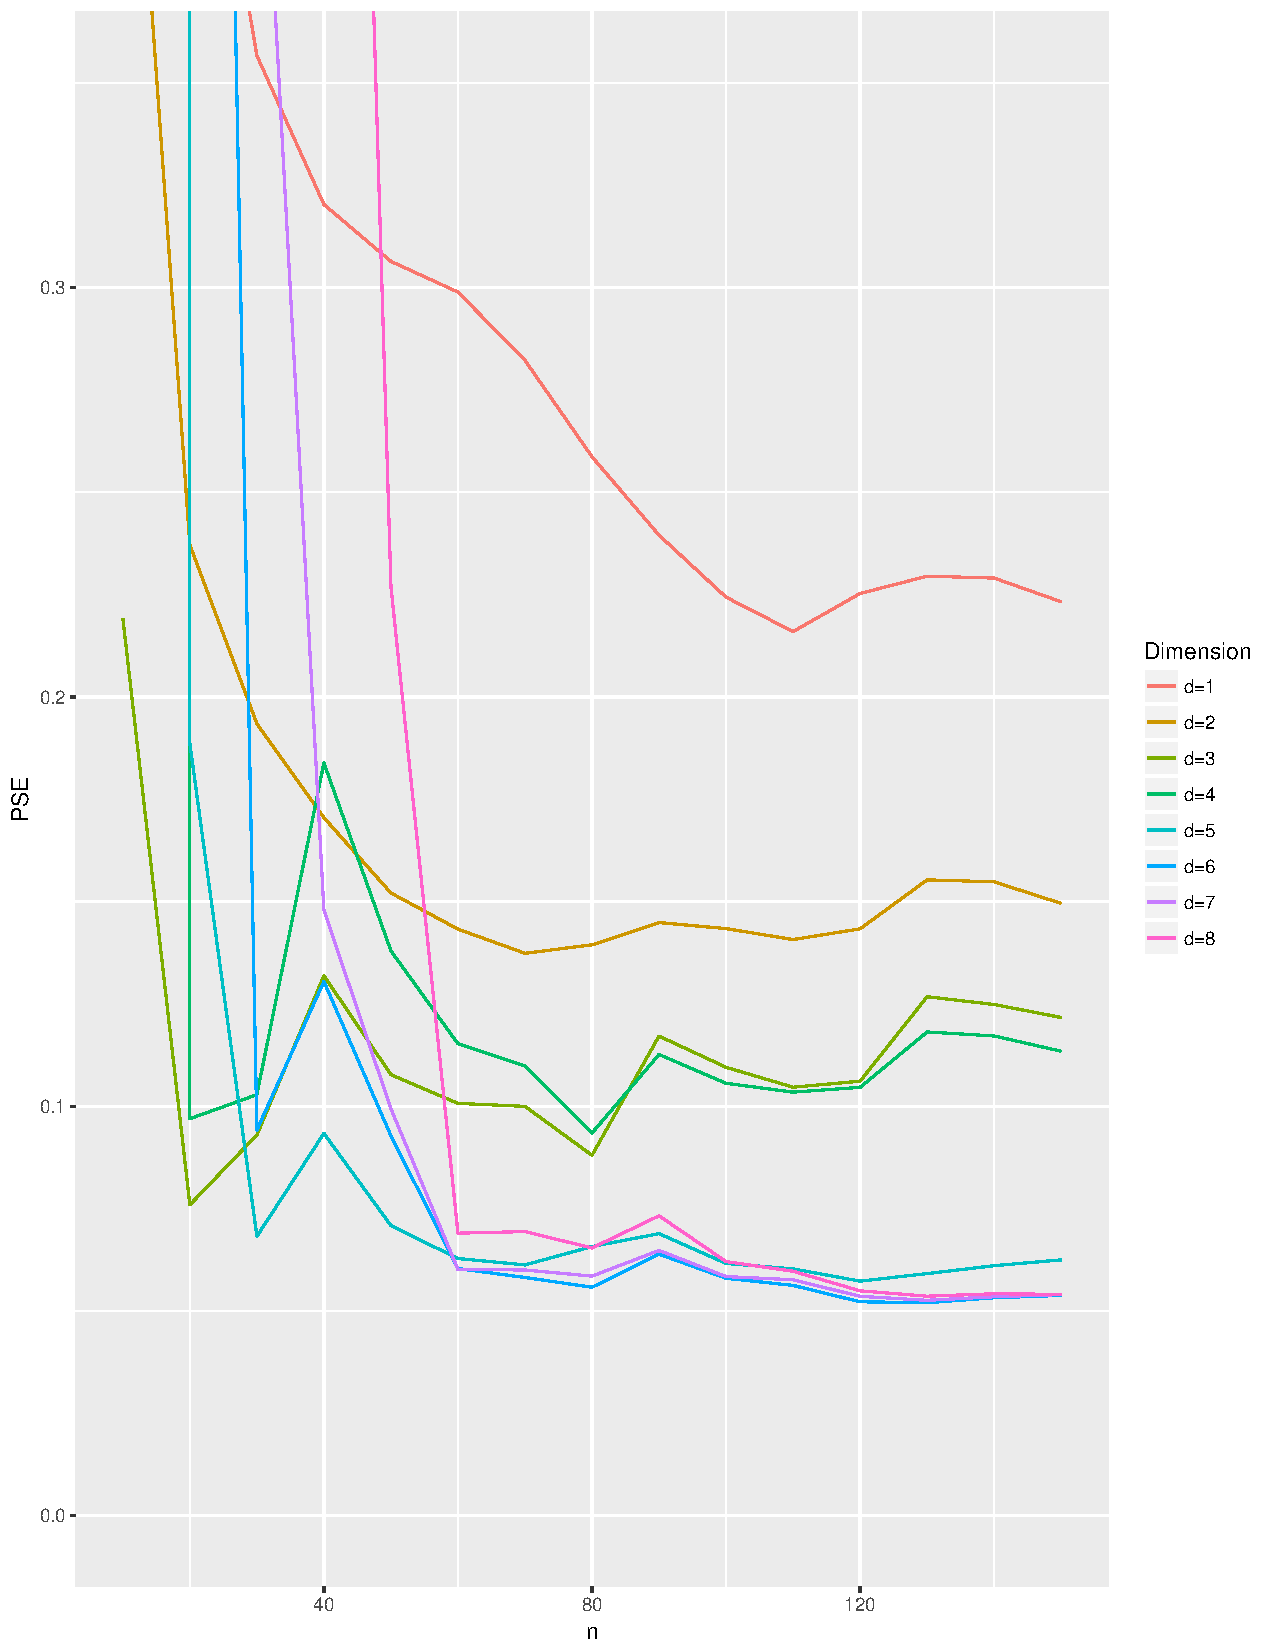
\includegraphics[width=0.8\textwidth, height= 6cm]{sim_plot.pdf}  
    \caption{The effect of the $n$ on $PSE$. From the graph we clearly see the optimal functional form relies on the sample size, $n$.}
    \label{fig:sim}{}
\end{figure}
 As expected, the PSE decreases as $n$ increases. Furthermore, the optimal degree increases with $n$. A linear model is best only for $n=10$. At $n=20$, a quadratic fit minimizes the PSE. However, by $n=30$ a fifth degree polynomial is best and remains so until $n=50$. Ultimately, a sixth degree polynomial performs very well and is not supplanted by a seventh degree polynomial until $n=90$. We note that an eighth degree polynomial never minimizes the PSE.


\section{Real Data Application}
\subsection{Geyser Data Example}

Consider a canonical regression problem: the waiting period of the Old Faithful geyser and a function  of the previous eruption duration.  Here, we demonstrate that the sieve estimator gives similar results as other nonparametric regression estimates, but with many fewer degrees of freedom. The \textit{faithful} dataset has 272 data points, which is small, but sufficient to demonstrate the sieve estimator. As in the simulation above, a polynomial basis is used.

First, consider a subset of the geyser data with only 40 data points.  Here, as expected, sieve estimators with a low dimension before the best. However, note that polynomials of low degree still perform better than simply a linear model.
\begin{figure}[h]
    \centering
    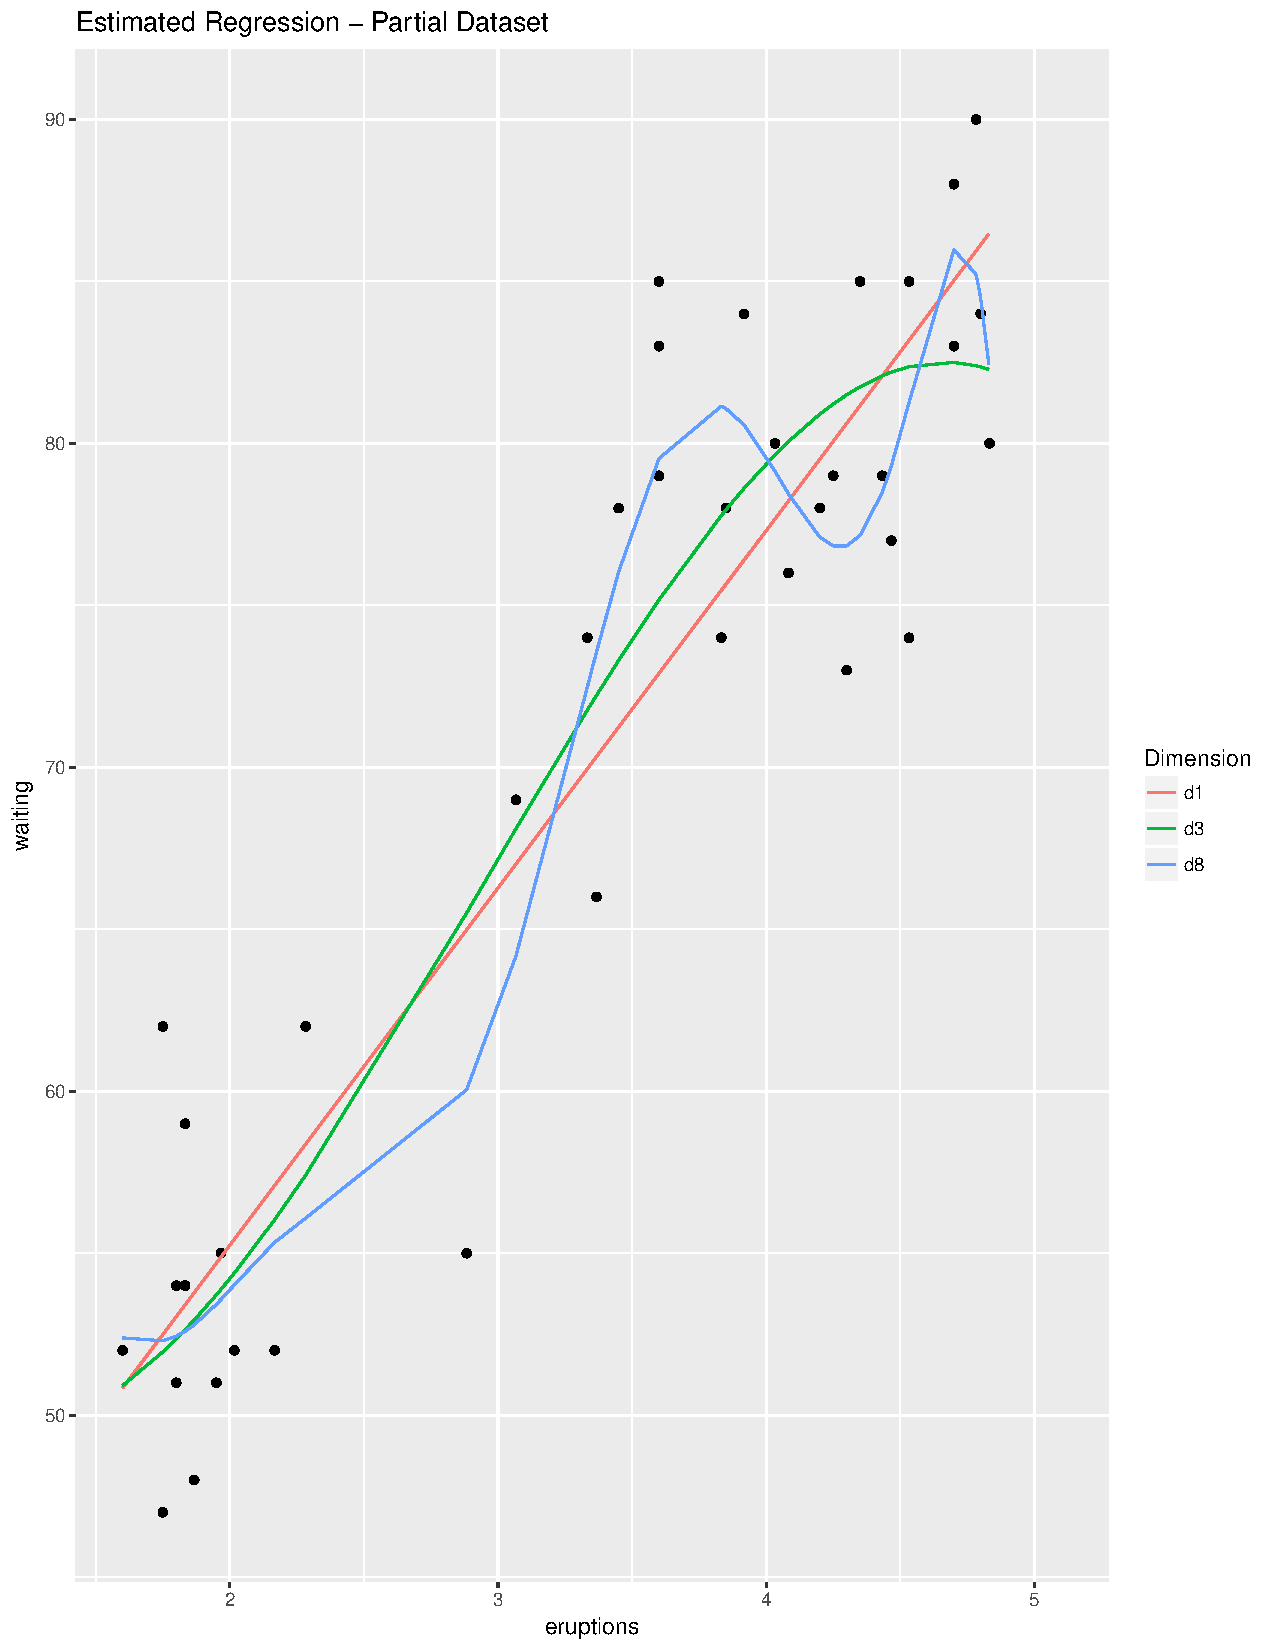
\includegraphics[width=0.45\textwidth, height = 6cm]{Geyser_Small_Data.pdf}
    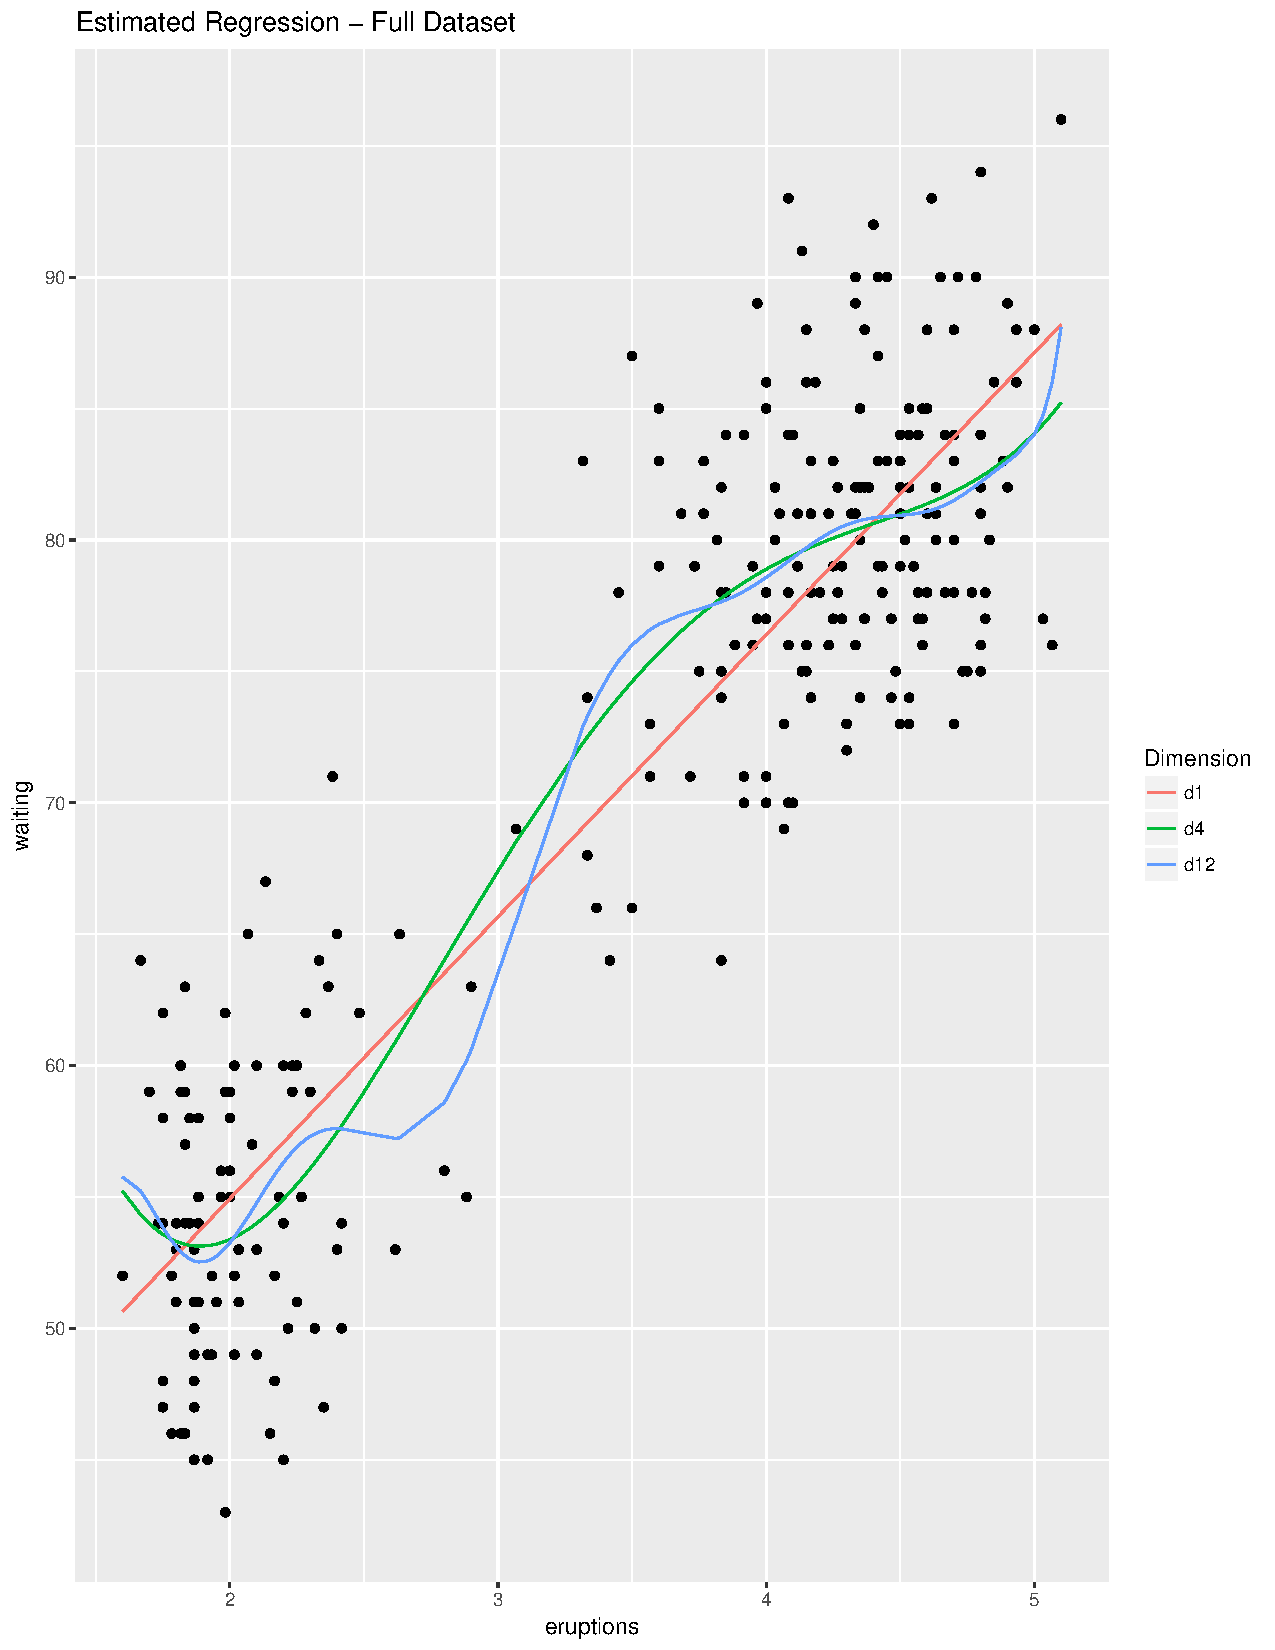
\includegraphics[width=0.45\textwidth, height = 6cm]{Geyser_Full.pdf}\\
    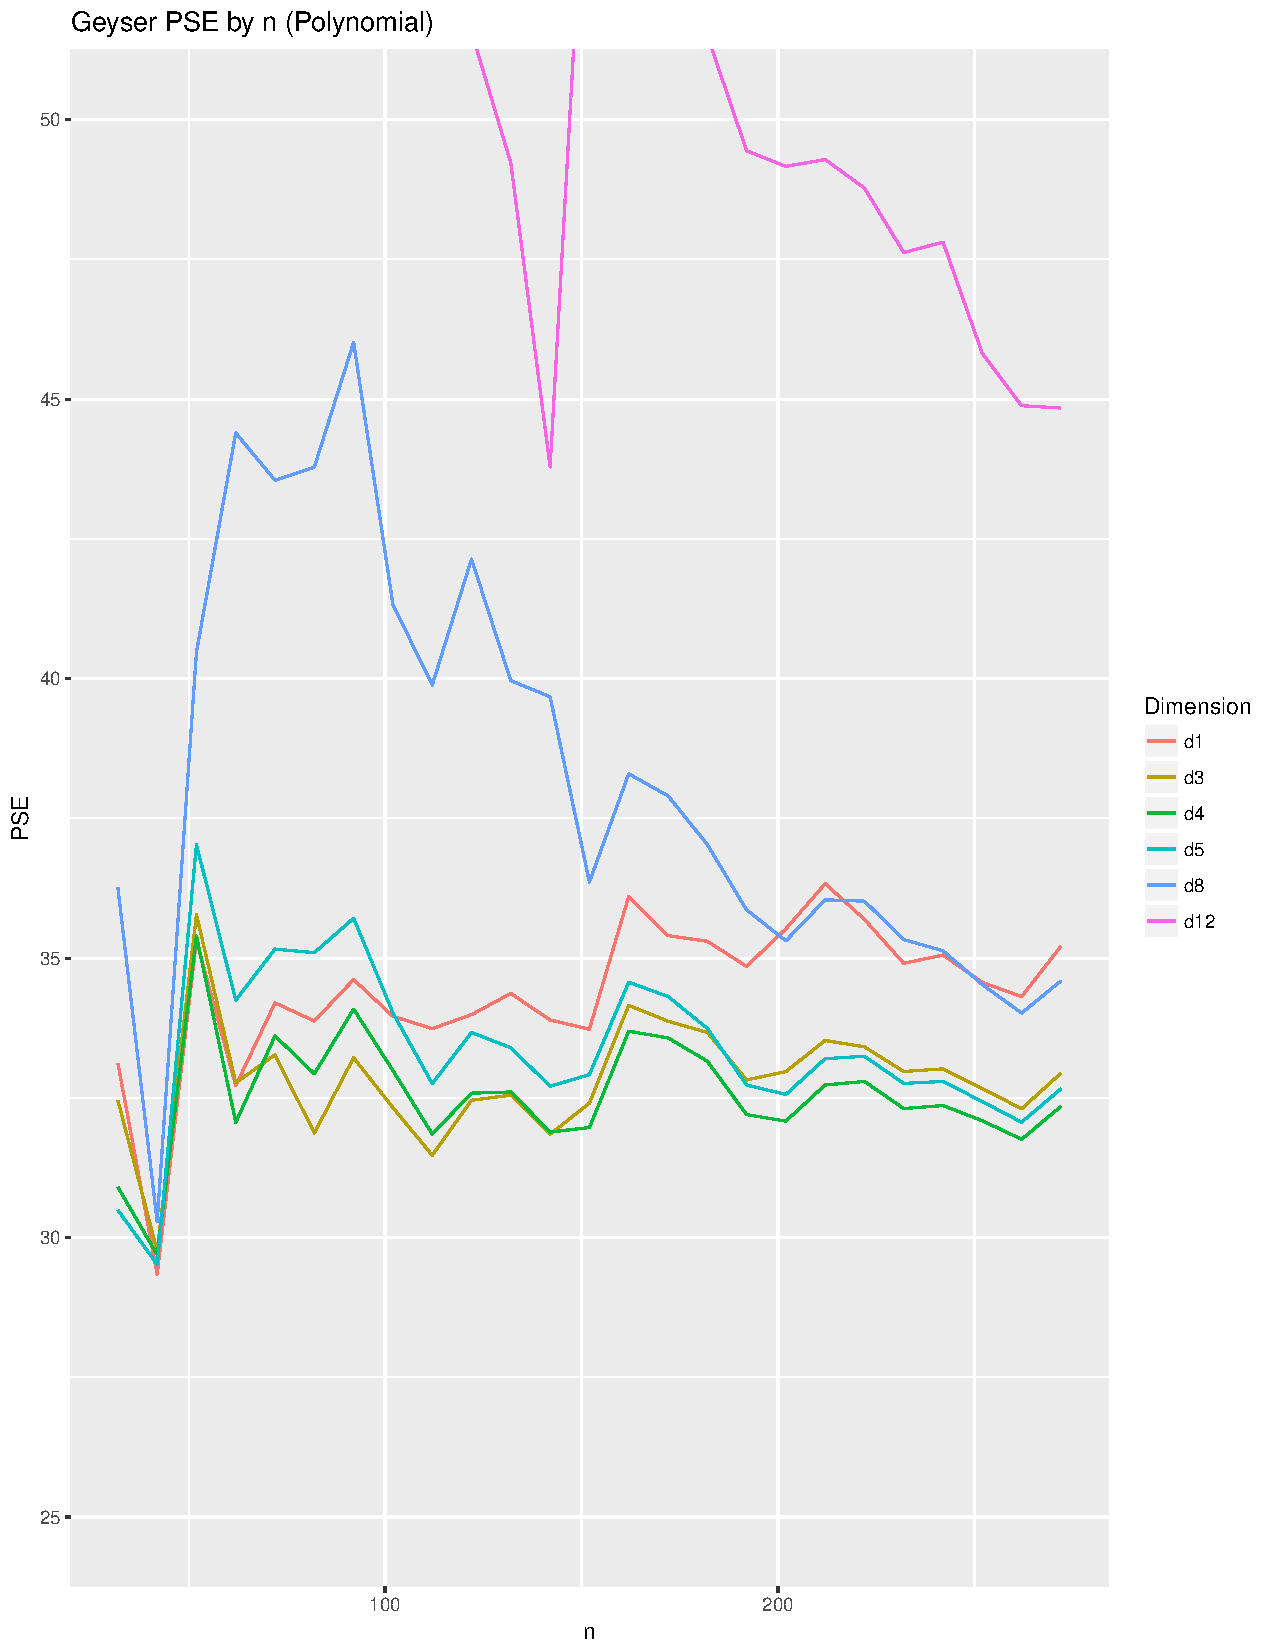
\includegraphics[width=0.45\textwidth, height = 6cm]{Geyser_PSE.pdf}\\
    \caption{Sieves Analysis of Geyser dataset. We see that increasing our sample size leads to differing optimal models}
    \label{fig:Geyser}{}
\end{figure}

With the full 272 data points, the optimal dimension is 4, which has increased from the case with only 40 data points. Note that the optimal dimension increases much more slowly than N. Again, if D grows too quickly (I.e. 11) then the data is overfit and the variance is large. 


\subsection{Econometric Example}

De Sa and Portugal apply sieve estimators to model a loss function of inflation and output gap for the Brazilian Central Bank and the Federal Reserve for their determination of interest rates.  The sieve estimator is chosen because the sieve estimator allows for global computation of the derivatives of the estimator. Therefore, a polynomial basis is a natural choice for the easy interpretation of derivatives in the model; specifically a Chebyshev Polynomial basis is used because the loss function is defined on $[-1,1]$.  A set of 14 variables is chosen to be the basis, and a sieve estimator is fit. If any of the coefficients of degree 3 or higher are significantly different than zero, then De Sa and Portugal would conclude third derivative is non-zero and therefore the loss function is asymmetric. 

In the sieve estimator, the cross term between inflation and the output gap is near zero, so the problem is separable into the inflation and output gap components. Based on the sieve estimator the Federal Reserve was more concerned about inflation than the output gap, which confirmed other studies. Furthermore, the sieve estimator does have non-zero third derivative with respect to inflation, and so it is concluded that the Federal Reserve was more concerned about high inflation than deflation from 1960-2011. However, when less data by considering only 1982-2011, then there was not significance to conclude that there was asymmetry.  

This example uses sieve estimators in a multivariate inferential context, which is a natural extension of the single dimensional estimator discussed in sections 2 and 3. However, the advantage of the sieve estimator is apparent by specifying a general, closed-form, global functional form which results in intuitive determination of parameters of interest in the economic model. 


\section{Conclusion}

In this report, we develop the methodology of a general sieve estimator, discuss the properties of a polynomial series sieve estimator, and explore data driven applications. Sieve estimators are general estimators and able to model many different classes of mean functions. Like other non parametric estimators, two key  choices are the choice of basis function, which is determined by properties of the problem, and the choice of dimension, which controls the complexity of the estimator.  We propose selecting the dimension through a cross validation scheme. Solving the polynomial series sieve estimator, after choosing the dimension and basis, is equivalent to solving ordinary least squares. With this property, we derive the MISE and justify the use of predicted squared error as a criterion to select the dimension. 

Furthermore, we evaluate the empirical use the sieve estimator through simulation and observed data sets. The simulation illustrates how the dimension of the estimator increases as the amount of data increases and the dimension grows much more slowly than N, which results in the asymptotic properties of the  MISE.  In the Old Faithful example, we show how a sieve estimator naturally incorporates additional data to better approximate the mean function with much less model complexity than other nonparametric regression estimators. 

Further exploration could be done by considering a penalized sieve estimator as a way to control model complexity. Little work has been on testing with sieve estimators, and the simple functional forms of the estimators may lead to useful results for global properties of the mean function. 


\section{References}
\nocite{*}
\printbibliography[heading=none]


\end{document} 

